\subsection{Interrelación Alumno Curso Académico - Reunión}

   \begin{description}
      \item[Definición] En esta interrelación se deja constancia de que un
      alumno puede participar en reuniones con su asesor durante un determinado
      curso académico.

      \item[Características] La interrelación presenta las siguientes
                             características:

         \begin{itemize}
            \item \textbf{Nombre:} AlCA-R
            \item \textbf{Tipo de la interrelación:} El tipo de entidad Reunión
                  es débil por identificación respecto al tipo de entidad Alumno
                  Curso Académico.
            \item \textbf{Cardinalidad de la interrelación:} 1:N
                  \begin{itemize}
                     \item Alumno Curso Académico: participa\_en (0,n)
                     \item Reunión: realizada\_a (1,1)
                  \end{itemize}
            \item \textbf{Número de atributos:} Ninguno.
         \end{itemize}

      \item[Diagrama] La figura \ref{diagramaAlCA-R} muestra el diagrama de la
                      interrelación.

      \item \begin{figure}[!ht]
            \begin{center}
            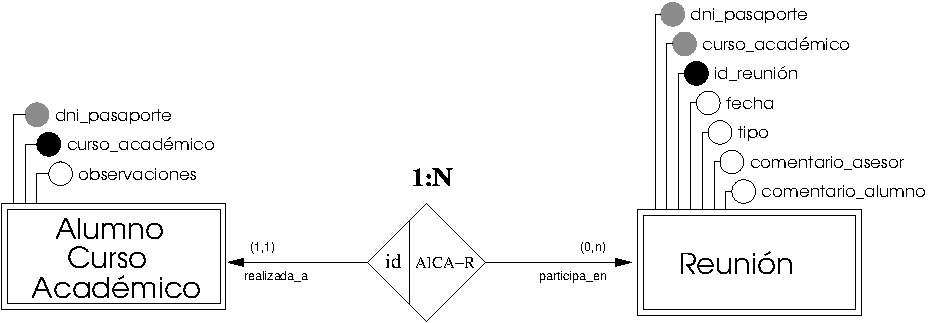
\includegraphics[]{07.Modelo_Entidad-Interrelacion/7.3.Analisis_Interrelaciones/diagramas/AlCA-R.pdf}
            \caption{Diagrama de la interrelación AlCA-R.}
            \label{diagramaAlCA-R}
            \end{center}
         \end{figure}

      \item[Ejemplo práctico del tipo de interrelación]

      \item \begin{center}
            \begin{tabular}{ | r r | }
            \hline
            \multicolumn{2}{ | c | }{\textbf{Tipo de interrelación AlCA-R}} \\
            \hline
            \textbf{Alumno Curso Académico} & \\
            dni\_pasaporte & 01234567A \\
            curso\_académico & 2008 \\
            \hline
            \textbf{Reunión} & \\
            dni\_pasaporte & 98765432Z \\
            curso\_académico & 2008 \\
            id\_reunión & 121 \\
            \hline
            \end{tabular}
         \end{center}
   \end{description}
